%
% design.tex
%
% Copyright (C) 2022 by SpaceLab.
%
% TTC 2.0 Critical Design Review
%
% This work is licensed under the Creative Commons Attribution-ShareAlike 4.0
% International License. To view a copy of this license,
% visit http://creativecommons.org/licenses/by-sa/4.0/.
%

%
% \brief Design slides.
%
% \author Gabriel Mariano Marcelino <gabriel.mm8@gmail.com>
% \author Miguel Boing <miguelboing13@gmail.com>
%
% \version 0.1.0
%
% \date 2022/07/28
%


\begin{frame}{Specifications}

    \begin{itemize}
        \item \textbf{Microcontroller}: MSP430F6659/MSP430F5659
        \item \textbf{Clock}: 32 MHz
        \item \textbf{Memories}:
        \begin{itemize}
            \item \textit{RAM}: 64 kB (SRAM)
            \item \textit{Flash}: 512 kB (code)
        \end{itemize}
        \item \textbf{Sensors}: Voltage, current and temperature
        \item \textbf{Modulation}: (G)FSK or (G)MSK
        \item \textbf{Baudrate}: 1200 to 9600 bps
        \item \textbf{Frequency}: 145-146 MHz, 435-438 MHz or 450 MHz bands
        \item \textbf{Protocol}: NGHam
        \item \textbf{Interfaces}: UART, I$^{2}$C and SPI
        \item \textbf{Mass}: 73 g
        \item PC-104 compatible
    \end{itemize}

\end{frame}

% #########################################################################
% #########################################################################

\begin{frame}{Electrical Block Diagram}

    \begin{figure}[!ht]
        \begin{center}
            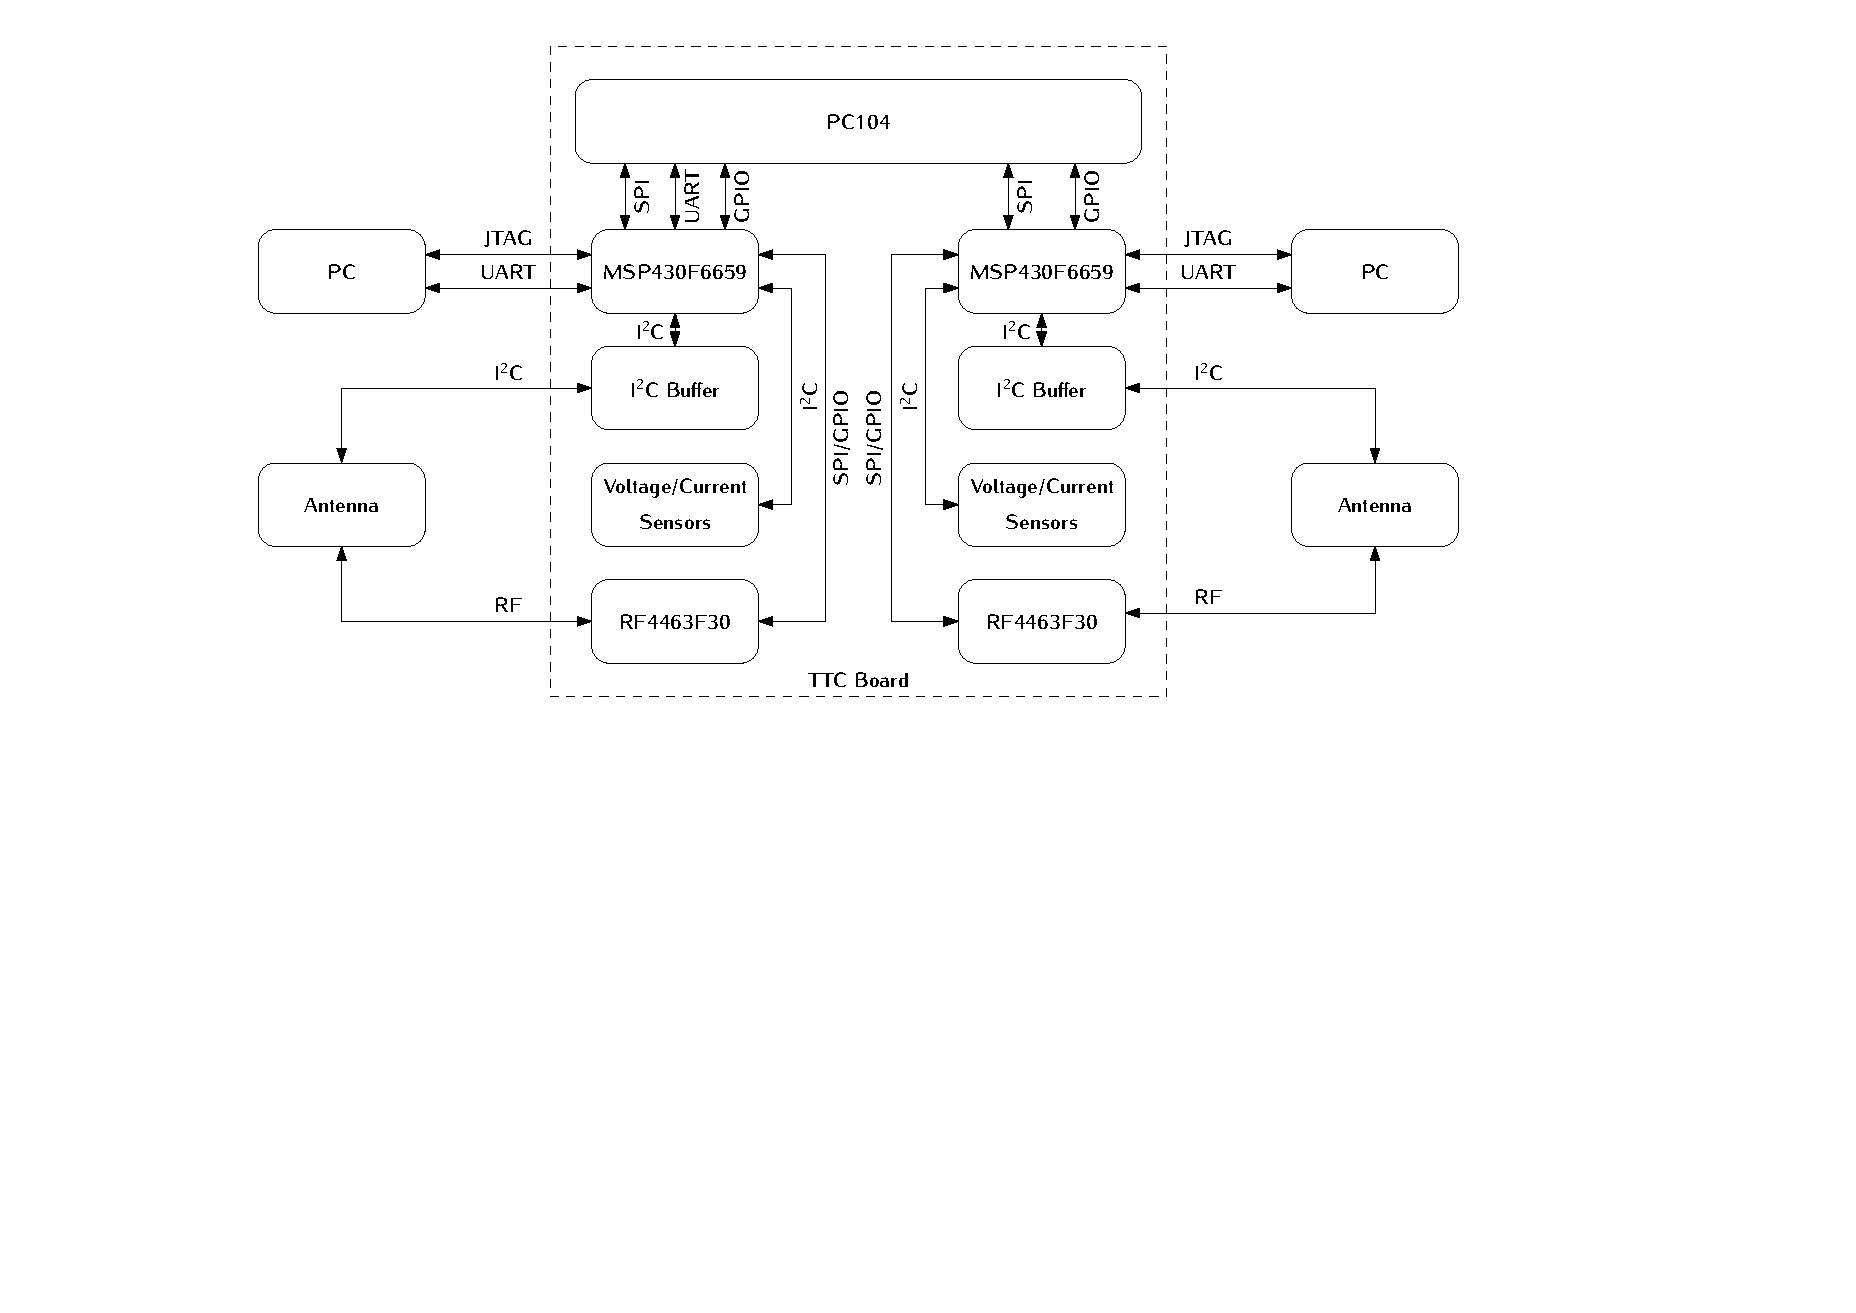
\includegraphics[width=11cm]{figures/hardware_diagram}
        \end{center}
    \end{figure}

\end{frame}

\begin{frame}{Schematics}

    Available at: \href{https://github.com/spacelab-ufsc/ttc2/tree/master/hardware/outputs/board_schematics}{\textcolor{blue}{\underline{https://github.com/spacelab-ufsc/ttc2}}}

    \begin{figure}[!ht]
        \begin{center}
            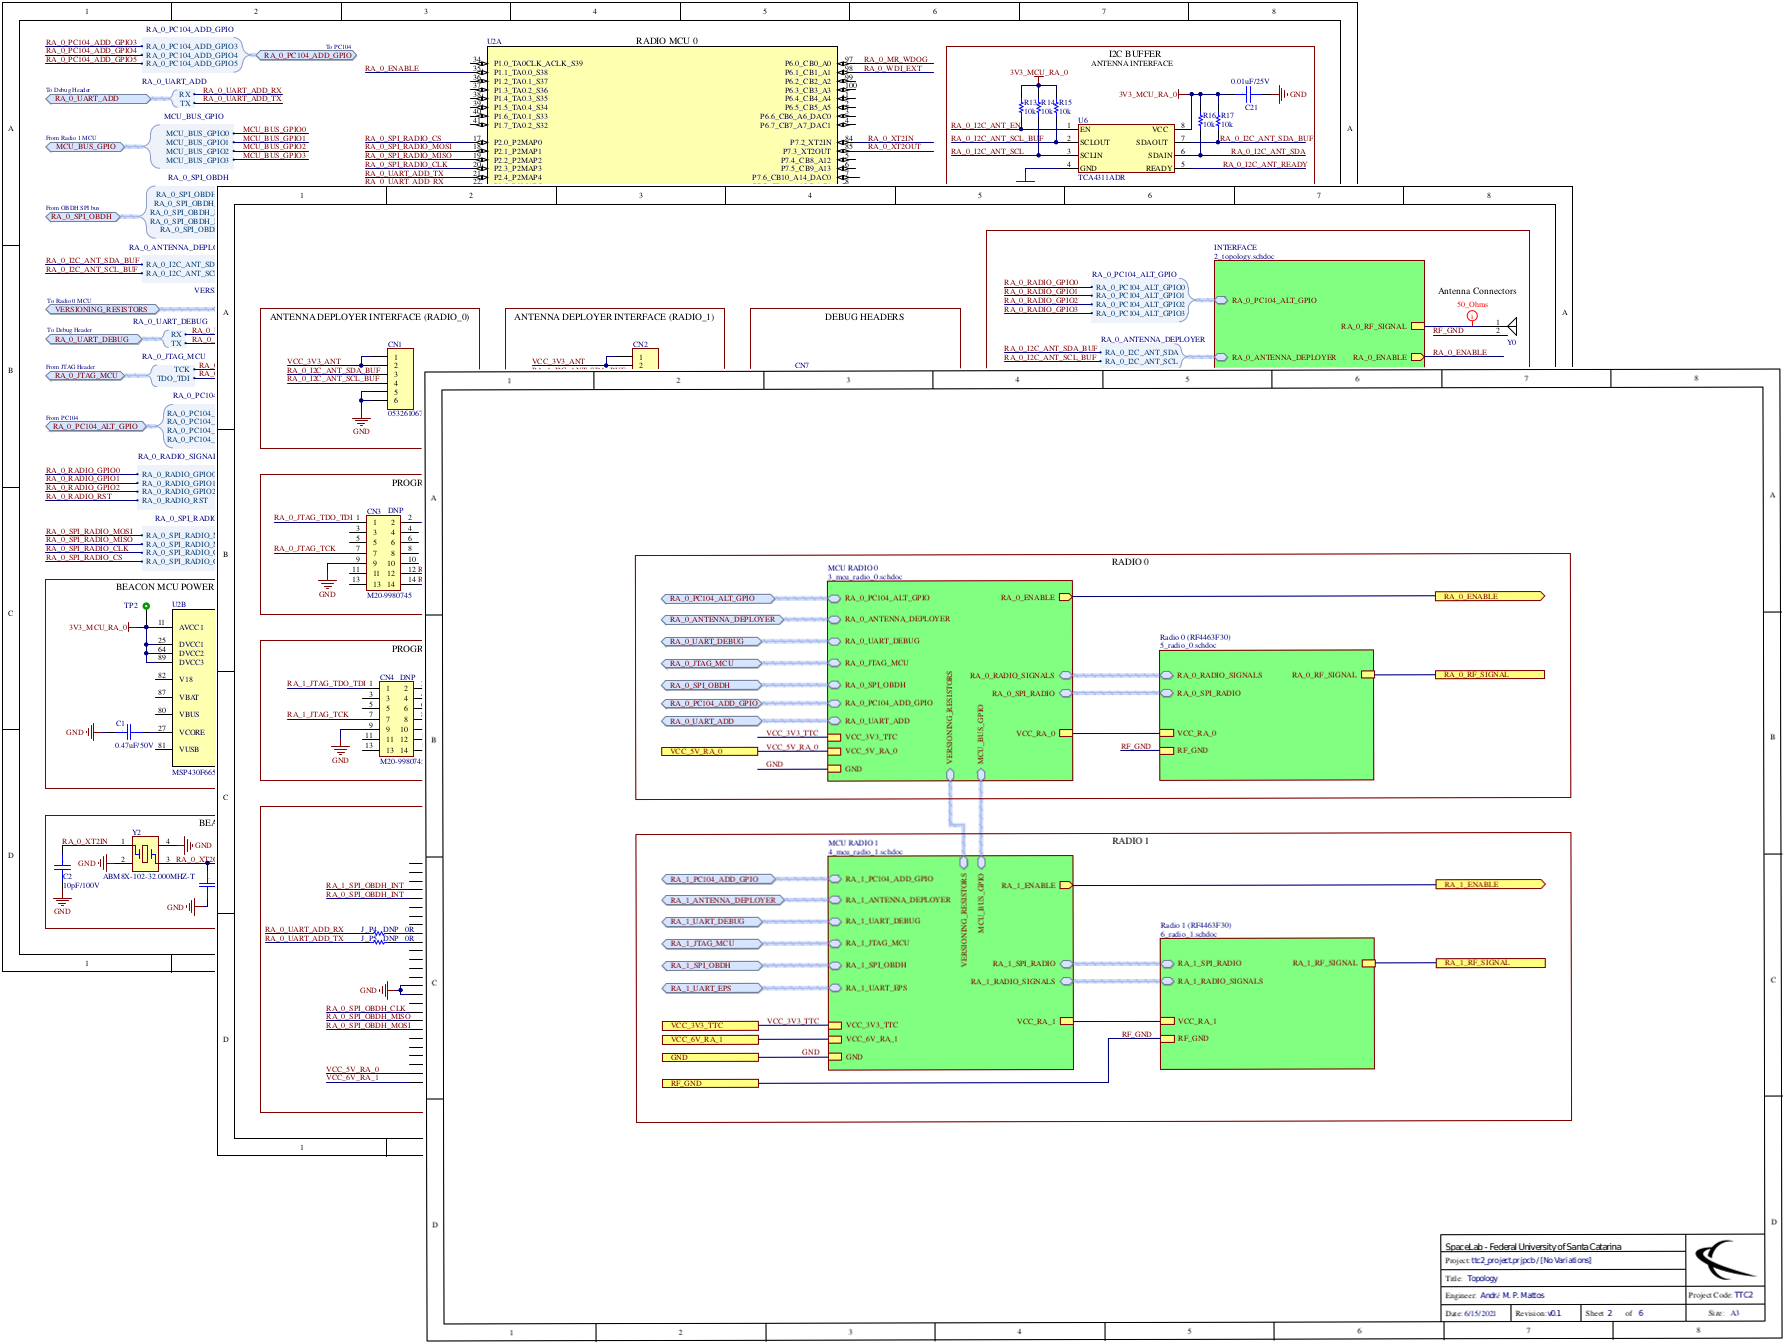
\includegraphics[width=8.5cm]{figures/ttc2-schematics.png}
        \end{center}
    \end{figure}

\end{frame}

\begin{frame}{PCB Layout}

    Available at: \href{https://github.com/spacelab-ufsc/ttc2/tree/master/hardware/sources}{\textcolor{blue}{\underline{https://github.com/spacelab-ufsc/ttc2}}}

    \begin{columns}[t]
        \begin{column}[t]{0.5\textwidth}
            \begin{figure}[!ht]
                \begin{center}
                    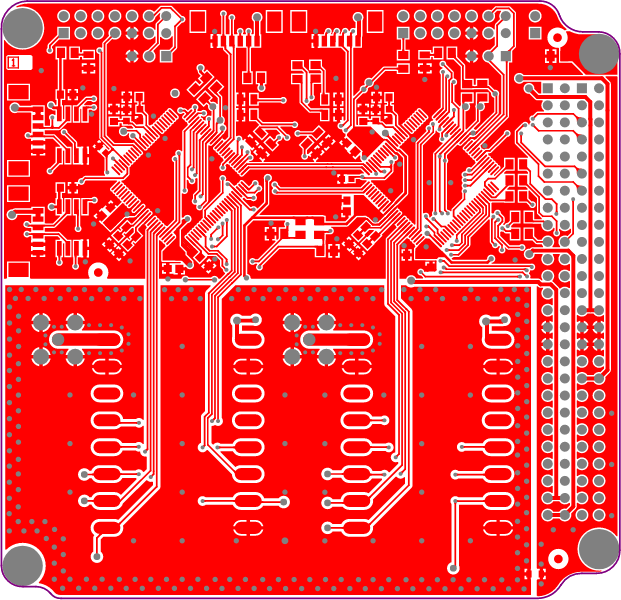
\includegraphics[width=5cm]{figures/ttc2-layout-top.png}
                \end{center}
                \caption{Top side}
            \end{figure}
        \end{column}
        \begin{column}[t]{0.5\textwidth}
            \begin{figure}[!ht]
                \begin{center}
                    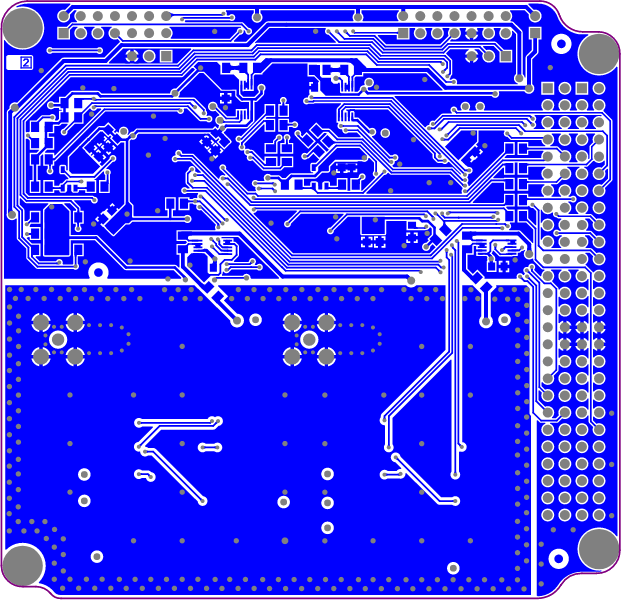
\includegraphics[width=5cm]{figures/ttc2-layout-bottom.png}
                \end{center}
                \caption{Bottom side}
            \end{figure}
        \end{column}
    \end{columns}

\end{frame}

\begin{frame}{3D Model}

    Available at: \href{https://github.com/spacelab-ufsc/ttc2/tree/master/hardware/outputs/board_3dmodels}{\textcolor{blue}{\underline{https://github.com/spacelab-ufsc/ttc2}}}

    \begin{figure}[!ht]
        \begin{center}
            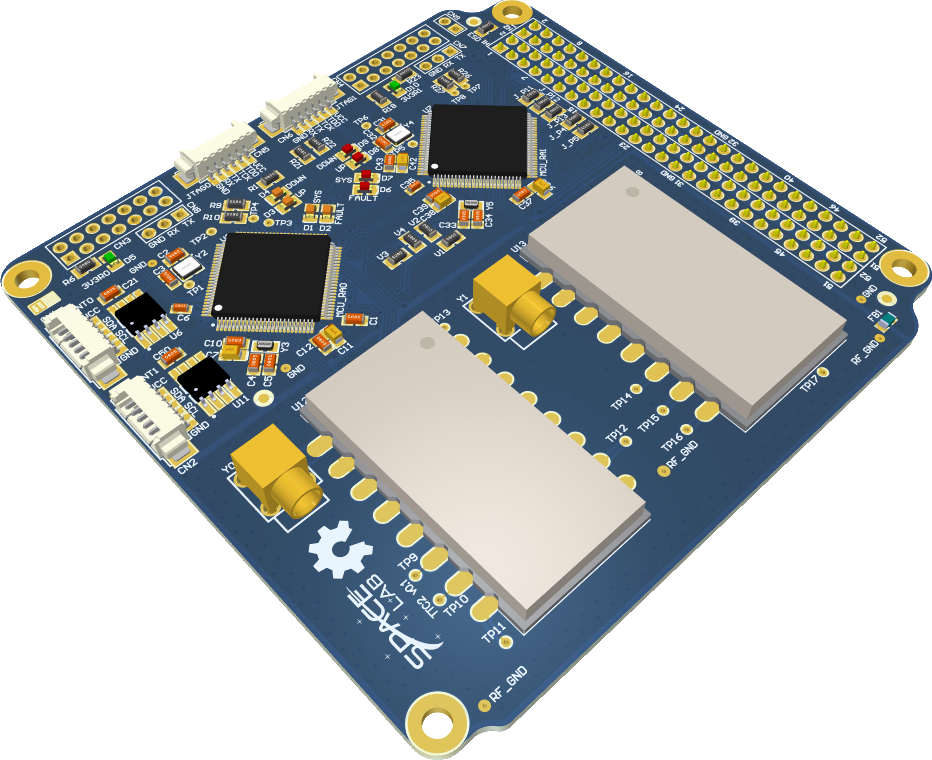
\includegraphics[width=7.5cm]{figures/ttc2_pcb_3d.png}
        \end{center}
    \end{figure}

\end{frame}

% #########################################################################
% #########################################################################

\begin{frame}{Power Consumption}

    \begin{itemize}
        \item Three separated voltage inputs: 3V3, 5V and 6V (microcontrollers and transceivers)
        \vspace{0.5cm}
        \item Power consumption\footnote{For one transceiver (there is two in TTC 2.0)}:
            \begin{itemize}
                \item Stand-by mode $\cong$ 83 mW
                \vspace{0.3cm}
                \item Transmission mode $\cong$ 2800 mW
                \vspace{0.3cm}
                \item Reception mode $\cong$ 163 mW
            \end{itemize}
    \end{itemize}

\end{frame}

% #########################################################################
% #########################################################################

\begin{frame}{Electrical Interfaces: PC-104}

\begin{table}[!h]\tiny
    \centering
    \begin{tabular}{cllll}
        \toprule[1.5pt]
        \textbf{Pin [A-B]} & \textbf{H1A}     & \textbf{H1B}     & \textbf{H2A}  & \textbf{H2B}  \\
        \midrule
        1-2                & -                & -                & -                & -                \\
        3-4                & -                & -                & -                & -                \\
        5-6                & -                & -                & RA\_1\_UART\_RX  & -                \\
        7-8                & GPIO\_6          & GPIO\_7          & RA\_1\_UART\_TX  & GPIO\_0          \\
        9-10               & RA\_1\_SPI\_INT  & RA\_1\_EN        & -                & -                \\
        11-12              & RA\_0\_SPI\_INT  & RA\_0\_EN        & RA\_1\_SPI\_MOSI & RA\_1\_SPI\_CLK  \\
        13-14              & -                & -                & RA\_1\_SPI\_CS   & RA\_1\_SPI\_MISO \\
        15-16              & -                & -                & -                & -                \\
        17-18              & -                & -                & -                & GPIO\_1          \\
        19-20              & -                & GPIO\_2          & -                & GPIO\_3          \\
        21-22              & -                & -                & -                & GPIO\_4          \\
        23-24              & -                & -                & -                & -                \\
        25-26              & -                & -                & -                & -                \\
        27-28              & -                & -                & VCC\_3V3         & VCC\_3V3         \\
        29-30              & GND              & GND              & GND              & GND              \\
        31-32              & GND              & GND              & GND              & GND              \\
        33-34              & -                & -                & -                & -                \\
        35-36              & RA\_0\_SPI\_CLK  & -                & VCC\_3V3\_ANT    & VCC\_3V3\_ANT    \\
        37-38              & RA\_0\_SPI\_MISO & -                & -                & -                \\
        39-40              & RA\_0\_SPI\_MOSI & RA\_0\_SPI\_CS   & -                & -                \\
        41-42              & -                & -                & -                & GPIO\_5          \\
        43-44              & -                & -                & -                & -                \\
        45-46              & -                & -                & -                & -                \\
        47-48              & -                & -                & -                & -                \\
        49-50              & VCC\_5V\_RA\_0   & VCC\_5V\_RA\_0   & -                & -                \\
        51-52              & VCC\_6V\_RA\_1   & VCC\_6V\_RA\_1   & -                & -                \\
        \bottomrule[1.5pt]
    \end{tabular}
    \label{tab:pc104-pins}
\end{table}

\end{frame}

\begin{frame}{Other Electrical Interfaces}

    \begin{table}[!htb]\tiny
        \centering
        \label{tab:icd}
        \begin{tabular}{lccl}
            \toprule[1.5pt]
            \textbf{Connector} & \textbf{Interface} & \textbf{Type} & \textbf{Pins} \\
            \midrule
            \multirow{6}{*}{CN1} & \multirow{6}{*}{I$^{2}$C} & \multirow{6}{*}{PicoBlade} & 3V3 \\
                                 &                           &                            & 3V3 \\
                                 &                           &                            & I2C\_SDA \\
                                 &                           &                            & I2C\_SCL \\
                                 &                           &                            & GND \\
                                 &                           &                            & GND \\
            \midrule
            \multirow{6}{*}{CN2} & \multirow{6}{*}{I$^{2}$C} & \multirow{6}{*}{PicoBlade} & 3V3 \\
                                 &                           &                            & 3V3 \\
                                 &                           &                            & I2C\_SDA \\
                                 &                           &                            & I2C\_SCL \\
                                 &                           &                            & GND \\
                                 &                           &                            & GND \\
            \bottomrule[1.5pt]
        \end{tabular}
    \end{table}

\end{frame}

\begin{frame}{Other Electrical Interfaces}

    \begin{table}[!htb]\tiny
        \centering
        \label{tab:icd}
        \begin{tabular}{lccl}
            \toprule[1.5pt]
            \textbf{Connector} & \textbf{Interface} & \textbf{Type} & \textbf{Pins} \\
            \midrule
            \multirow{14}{*}{CN3} & \multirow{14}{*}{JTAG} & \multirow{14}{*}{Pin Header} & TDO\_TDI \\
                                  &                        &                              & 3V3 \\
                                  &                        &                              & None \\
                                  &                        &                              & None \\
                                  &                        &                              & None \\
                                  &                        &                              & None \\
                                  &                        &                              & TCK \\
                                  &                        &                              & None \\
                                  &                        &                              & GND \\
                                  &                        &                              & None \\
                                  &                        &                              & None \\
                                  &                        &                              & UART\_TX \\
                                  &                        &                              & None \\
                                  &                        &                              & UART\_RX \\

            \bottomrule[1.5pt]
        \end{tabular}
    \end{table}

\end{frame}

\begin{frame}{Other Electrical Interfaces}

    \begin{table}[!htb]\tiny
        \centering
        \label{tab:icd}
        \begin{tabular}{lccl}
            \toprule[1.5pt]
            \textbf{Connector} & \textbf{Interface} & \textbf{Type} & \textbf{Pins} \\
            \midrule
            \multirow{14}{*}{CN4} & \multirow{14}{*}{JTAG} & \multirow{14}{*}{Pin Header} & TDO\_TDI \\
                                  &                        &                              & 3V3 \\
                                  &                        &                              & None \\
                                  &                        &                              & None \\
                                  &                        &                              & None \\
                                  &                        &                              & None \\
                                  &                        &                              & TCK \\
                                  &                        &                              & None \\
                                  &                        &                              & GND \\
                                  &                        &                              & None \\
                                  &                        &                              & None \\
                                  &                        &                              & UART\_TX \\
                                  &                        &                              & None \\
                                  &                        &                              & UART\_RX \\

            \bottomrule[1.5pt]
        \end{tabular}
    \end{table}

\end{frame}

\begin{frame}{Other Electrical Interfaces}

    \begin{table}[!htb]\tiny
        \centering
        \label{tab:icd}
        \begin{tabular}{lccl}
            \toprule[1.5pt]
            \textbf{Connector} & \textbf{Interface} & \textbf{Type} & \textbf{Pins} \\
            \midrule
            \multirow{6}{*}{CN5} & \multirow{6}{*}{JTAG} & \multirow{6}{*}{PicoBlade} & 3V3 \\
                                 &                       &                            & TDO\_TDI \\
                                 &                       &                            & TCK \\
                                 &                       &                            & UART\_TX \\
                                 &                       &                            & UART\_RX \\
                                 &                       &                            & GND \\
            \midrule
            \multirow{6}{*}{CN6} & \multirow{6}{*}{JTAG} & \multirow{6}{*}{PicoBlade} & 3V3 \\
                                 &                       &                            & TDO\_TDI \\
                                 &                       &                            & TCK \\
                                 &                       &                            & UART\_TX \\
                                 &                       &                            & UART\_RX \\
                                 &                       &                            & GND \\
            \midrule
            \multirow{3}{*}{CN7} & \multirow{3}{*}{UART} & \multirow{3}{*}{PinHeader} & TX \\
                                 &                       &                            & RX \\
                                 &                       &                            & GND \\
            \midrule
            \multirow{3}{*}{CN8} & \multirow{3}{*}{UART} & \multirow{3}{*}{PicoBlade} & TX \\
                                 &                       &                            & RX \\
                                 &                       &                            & GND \\
            \midrule
            \multirow{2}{*}{CN9} & \multirow{2}{*}{Jumper} & \multirow{2}{*}{Pin Header} & 3V3 \\
                                 &                         &                      & - \\
            \bottomrule[1.5pt]
        \end{tabular}
    \end{table}

\end{frame}

\begin{frame}{Other Electrical Interfaces}

    \begin{table}[!htb]\tiny
        \centering
        \label{tab:icd}
        \begin{tabular}{lccl}
            \toprule[1.5pt]
            \textbf{Connector} & \textbf{Interface} & \textbf{Type} & \textbf{Pins} \\
            \midrule
            \multirow{2}{*}{Y0} & \multirow{2}{*}{RF} & \multirow{2}{*}{MCX} & RF\_SIGNAL \\
                                &                     &                      & RF\_GND \\
            \midrule
            \multirow{2}{*}{Y1} & \multirow{2}{*}{RF} & \multirow{2}{*}{MCX} & RF\_SIGNAL \\
                                &                     &                      & RF\_GND \\
            \bottomrule[1.5pt]
        \end{tabular}
    \end{table}

\end{frame}

\begin{frame}{Dimensions}

    \begin{figure}[!ht]
        \begin{center}
            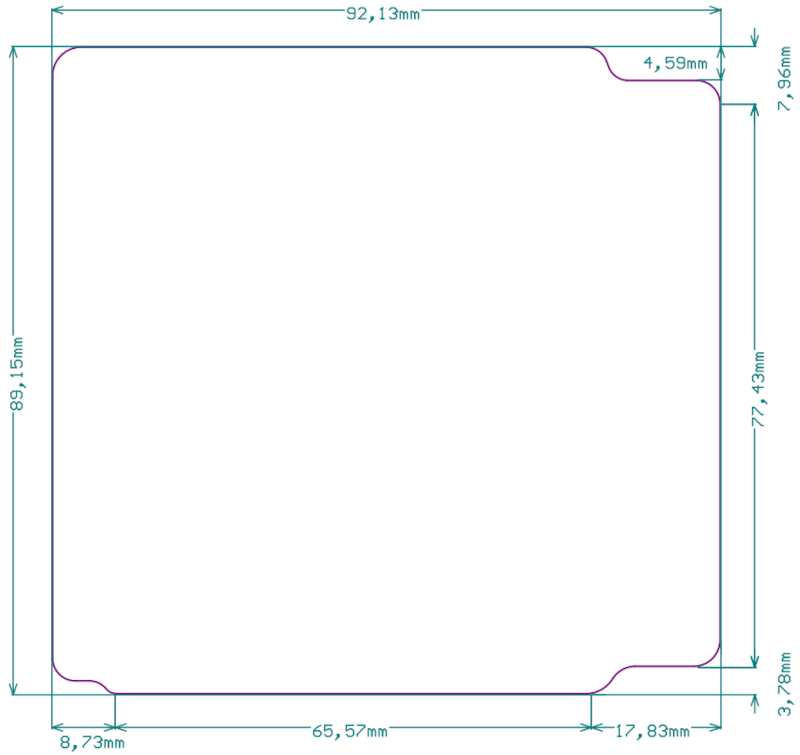
\includegraphics[width=7.5cm]{figures/board-dimensions.png}
        \end{center}
    \end{figure}

\end{frame}

\begin{frame}{Voltage/Current Sensors}

    \begin{itemize}
        \item Voltage, current and power sensor
        \vspace{0.3cm}
        \item Quantity: 4 (one per radio module and one per microncontroller circuit)
        \vspace{0.3cm}
        \item Texas Instruments INA226AQDGSRQ1
        \vspace{0.3cm}
        \item I$^{2}$C Interface
        \vspace{0.3cm}
    \end{itemize}


\end{frame}

\begin{frame}{External Watchdog}

    \begin{itemize}
        \item IC: Texas Instruments TPS3823
        \vspace{0.5cm}
        \item Voltage monitor with a watchdog timer feature
        \vspace{0.5cm}
        \item Timeout period: $1600\ ms$
        \vspace{0.5cm}
        \item Reset period: $100\ ms$
    \end{itemize}

\end{frame}

\begin{frame}{Transceiver}

    \begin{itemize}
        \item \href{https://www.nicerf.com/products/detail/1w-rf-module-rf4463f30.html}{\textcolor{blue}{\underline{NiceRF RF4463F30}}}
        \item Based on \href{https://www.silabs.com/wireless/proprietary/ezradiopro-sub-ghz-ics/device.si4463?tab=specs}{\textcolor{blue}{\underline{Si4463}}} transceiver
        \item Integrated power amplifier and RF switch (single antenna)
        \item Half-Duplex
        \item Output power: 30 dBm
        \item SPI Interface
    \end{itemize}
    \begin{figure}[!ht]
        \begin{center}
            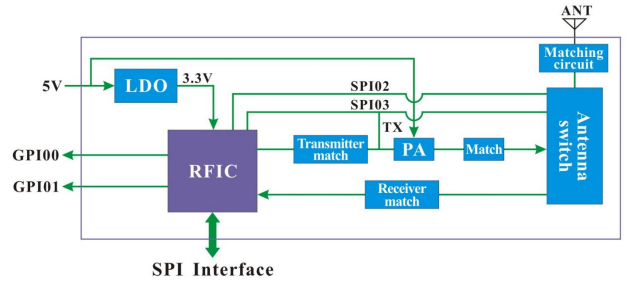
\includegraphics[width=10cm]{figures/rf4463f30-block-diagram.png}
        \end{center}
    \end{figure}

\end{frame}

\begin{frame}{Flight Model Specs. and Preparation}

    \begin{itemize}
        \item \textbf{PCB specs.}: IPC 6012 Class 3
        \vspace{0.3cm}
        \item \textbf{PCB thickness}: 1,6 mm
        \vspace{0.3cm}
        \item \textbf{Material}: TG170 FR-4
        \vspace{0.3cm}
        \item \textbf{Surface finish}: ENIG
        \vspace{0.3cm}
        \item \textbf{Board finish}: Conformal coating application
    \end{itemize}

\end{frame}
